\chapter{Traditional ML Pipeline and Features}
Traditionally, we use hand-designed node, link, graph level features to transform the graph into series of features, then feed into the machine learning model. 
\section{Node Level Features} 
Here are some important-based node features (degree, centrality) and structur-based node features (degree, clustering coefficient, graphlet count vector). 

\subsection{Node Degree}
Node degree $k_u$ just the number of edges the node $u$ has. 

\subsection{Node Centrality}
Node centrality tries to captude the node importance. \\
\par 

\textbf{Eigenvector centrality}:\\
We can model the centrality of a node $v$ as the sum of the centrality of neighboring nodes. i.e.: 
    \begin{align*}
        c_V = \frac{1}{\lambda} \sum_{u\in N(v)}c_u
    \end{align*}
    \begin{itemize}
        \item here $\lambda$ is the normalizing constant. 
    \end{itemize}
Turns out we can re-write it as matrix form $\lambda c_v = Ac$ where $c$ is the centrality vector, $A$ is the adjacency matrix, and $\lambda$ is the eigenvalue. This way we have the eigenvector $c_{max}$ correlated with the largest eigenvalue $\lambda_{max}$ to be the centrality measure. \\
\par

\textbf{Betweenness centrality}:\\
A node is important if it lies on many shortest path between other nodes. So we have 
    \begin{align*}
        c_v = \sum_{s \neq v \neq t} \frac{\textrm{shortest path between $s$ and $t$ that contain $v$}}{\textrm{shortest path between $s$ and $t$}}
    \end{align*}
\\
\par

\textbf{Closeness centrality}:\\
A node is important if it has small shortest path lengths to all other nodes. 
    \begin{align*}
        c_v = \frac{1}{\sum_{u\neq v}\textrm{shortest path length between $u$ and $v$}}
    \end{align*}


\subsection{Node Clustering Coefficient}
Node clustering coefficient measures how connected $v$'s neighboring nodes are: 
    \begin{align*}
        e_v = \frac{\textrm{\#(edges among neighboring nodes)}}{{k_v \choose 2}}
    \end{align*}
    \begin{itemize}
        \item $k_v$ is the degree of the node $v$
    \end{itemize}

\subsection{Node Graphlets \& GDV}
Graphlets are small subgraphs that describe network structure around node $u$. Graphlets are rooted connected induced non-isomorphic subgraphs. Below shows all graphlets of a fully connected graphs with 5 nodes. Notice the numbering on the subgraphs. Since graphlets are rooted, so the nodes position matters. e.g.: in subgraph G1, a node can either be the boarder node, or the central node. \\
\begin{figure}[H]
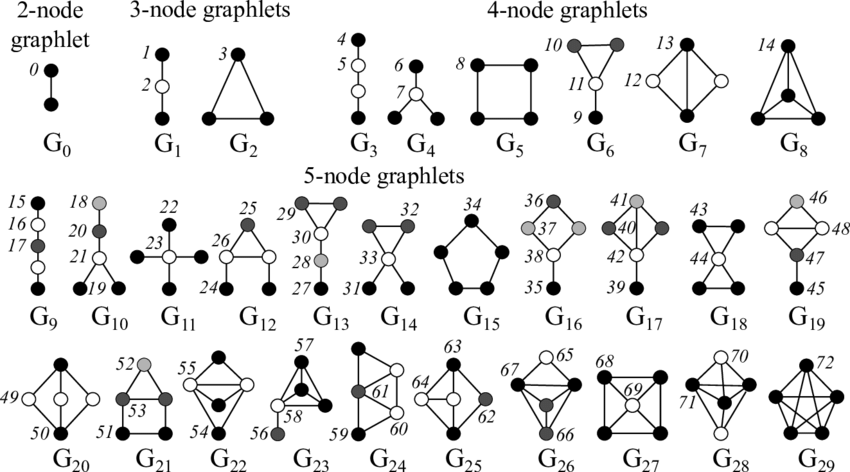
\includegraphics[width=12cm, height=6cm]{images/001_graphlets.png}
\end{figure}
Graphlet Degree Vector (GDV) is a count vector of graphlets rooted at a given node. I.e.: at index $i$, the value of the vector is the number of times node $u$ involved in graphlet configuration $i$. 




\section{Link Level Features}
Generally, we want to predict edges in two ways: 1) assume the graph is incomplete and edges are missing at random, 2) Given $G[t_0, t_0']$ a graph defined by edges up to time $t_0'$, output a ranked list $L$ of edges that are not in $G[t_0, t_0']$ but would appear in time $G[t_1, t_1']$. We can do this by computing a score between each node $c(u,v)$, and use the top scores as the predicted new edge.\\
Link level features can be based on distance, local neighborhood overlap, and global neighborhood overlap.\\

\subsection{Link Distance Based Features} 
Shortest-path distance between two nodes. 


\subsection{Local Neighborhood Overlap}
These set of features aim to captures number of neighboring nodes shared between two nodes $v_1$ and $v_2$. \\
\textbf{Common neighbors}
    \begin{align*}
        |N(v_1) \cap N(v_2)|
    \end{align*}
\\ 
\par

\textbf{Jaccard's coefficient}
    \begin{align*}
        \frac{|N(v_1) \cap N(v_2)|}{|N(v_1) \cup N(v_2)|}
    \end{align*}
\\
\par

\textbf{Adamic-Adar index}
    \begin{align*}
        \sum_{u\in N(v_1) \cap N(v_2)} \frac{1}{\log(k_u)}
    \end{align*}


\subsection{Global Neighborhood Overlap}
If two nodes do not have any neighbors in common, the metric is always 0. But two nodes could still be potentially connected in the future. So we now try to consider the entire graph. If the graph is undirected, we can calculate number of paths (strictly speaking, walks) of length $K$ be 
    \begin{align*}
        P^{(K)} = A^k
    \end{align*}
    \begin{itemize}
        \item $A$ is the adjacency matrix
        \item $A^k_{uv}$ entry is the number of walk of length $k$ between node $u$ and $v$
    \end{itemize}
The katz index counts the number of paths of all lengths between a given pair of nodes. So it can be calculated as 
    \begin{align*}
        & S_{v_1v_2} = \sum_{l=1}^\infty \beta^l A^l_{v_1v_2} \\
        & S = \sum_{i=1}^\infty \beta^iA^i = (I -\beta A)^{-1}-I = \sum_{i=0}^\infty \beta^i A^i
    \end{align*}
    \begin{itemize}
        \item $\beta$ is discount factor
    \end{itemize}
    
\section{Graph Level Features} 
Graph level features aims to characterize the structure of an entire graph. Graph kernel is a function $K(G, G')\in \mathbb{R}$ that takes in two graphs, and return a number measures similarity between two graphs. So the kernel matrix $K$ for a series of graphs must always be positive semidefinite. As a result, there exists a feature representation $\phi(\cdot)$ such that $K(G,G') = \phi(G)^T\phi(G')$. Once the kernel is defined, we can use reguar ML models such as kernel SVM. 

\subsection{Graphlet Kernel}
Goal: Design graph feature vector $\phi(G)$ using bag of words approach. We want to count the number of different graphlets (here it means non-rooted induced subgraph, and nodes do not need to be connected). So formally, given graph $G$ and a graphlet list $(g_1, g_2, ..., g_{n_k})$, define the graphlet count vector $f_G\in \mathbb{R}^{n_k}$ as 
    \begin{align*}
        (f_G)_i = \#(g_i \in G) \textrm{ for $i=1,2,...,n_k$ }
    \end{align*}
    \begin{itemize}
        \item Here $k$ denotes the number of nodes in the graphlet. E.g.: when $k=3$, there are 4 possible graphlet. 
    \end{itemize}
For example: 
    \begin{figure}[H]
    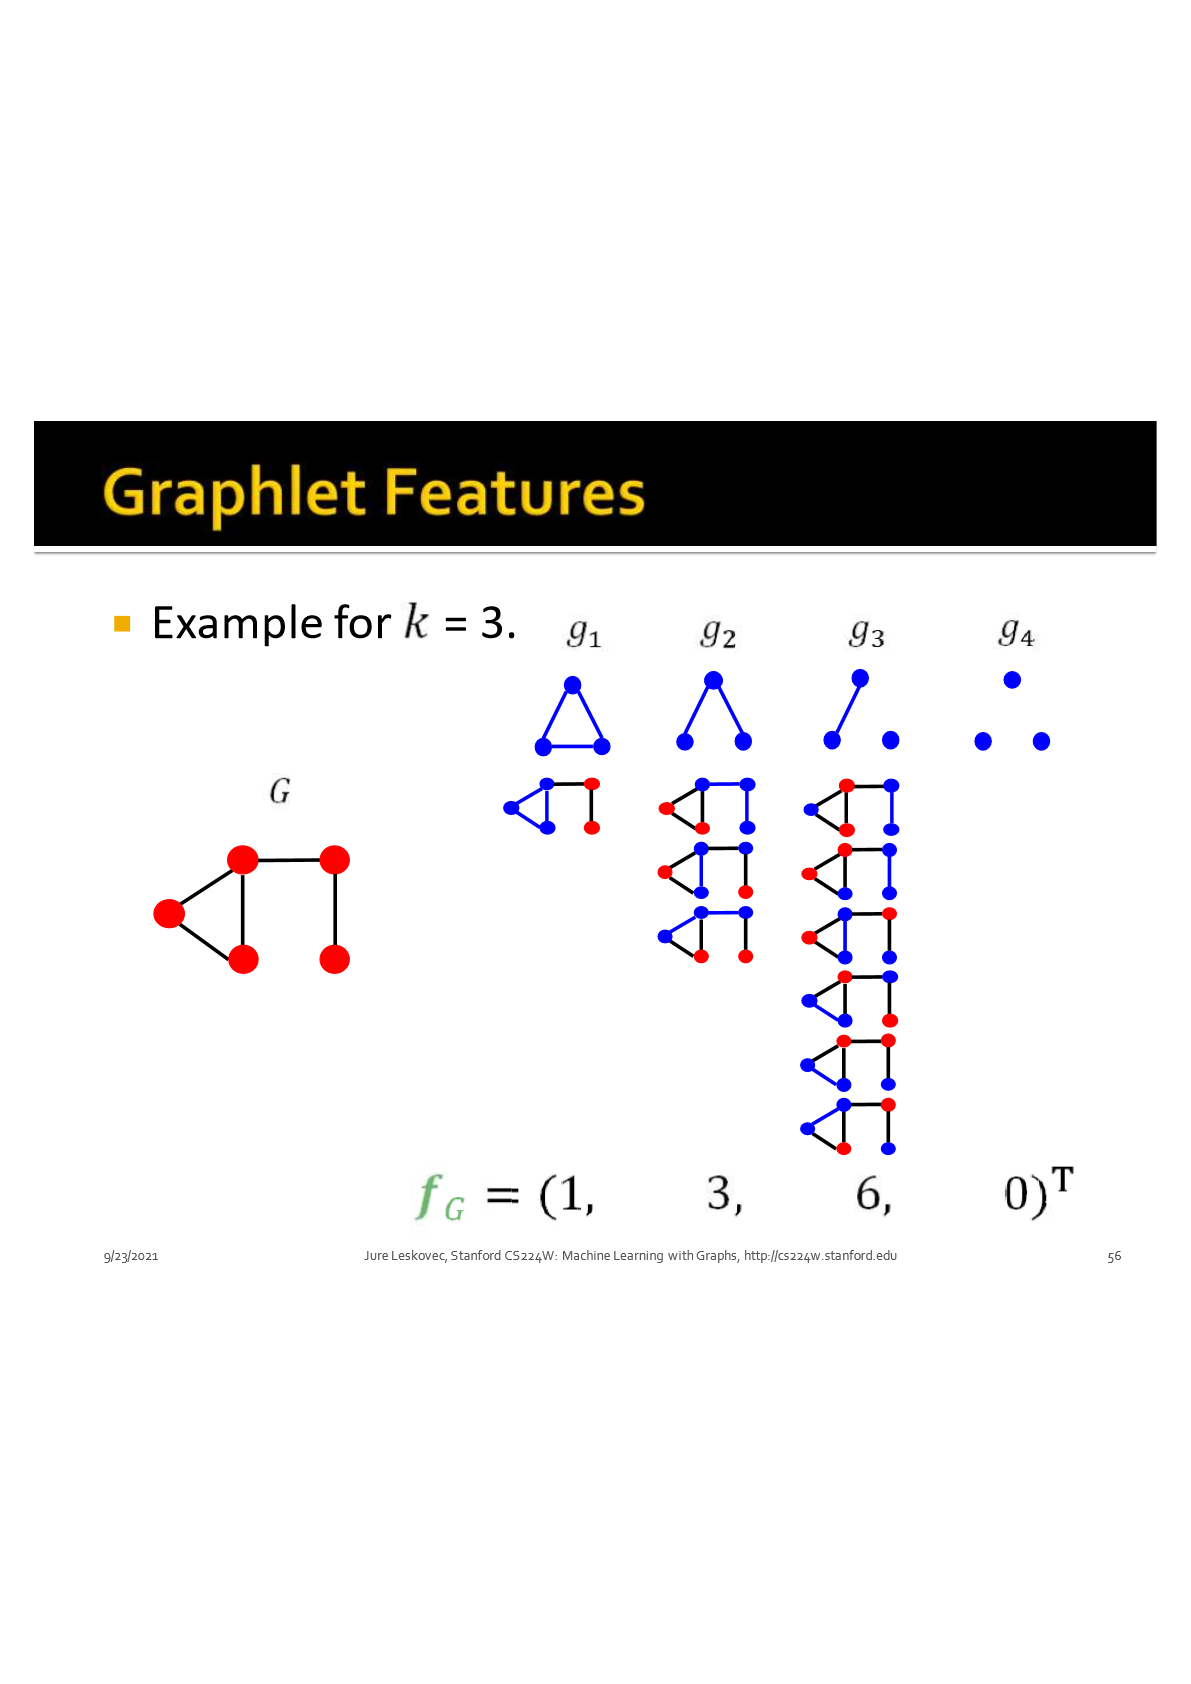
\includegraphics[width=10cm, height=10cm]{images/002_graphlet_kernel.png}
    \end{figure}
Given two graphs $G$ and $G'$, the graphlet kernel is computed using normalized feature vector as 
    \begin{align*}
        &K(G,G') = h_G^T h_{G'}\\
        &h_G = \frac{f_g}{Sum(f_G)}
    \end{align*}

\subsection{Weisfeiler-Lehman Kernel}
Use neighborhood structure to iteratively encirch node vocabulary. We do it through color refine algorithm.Given a graph $G$ with a set of nodes $V$. 
    \begin{enumerate}
        \item Assian an initial color $c^{(0)}(v)$ to each node $v$. 
        \item Iteratively refine node colors by $c^{(k+1)}(v) = HASH(c^{(k)}(v),\{c^{(k)}(u)\}_{u \in N(v)})$ (Hash function maps different input to different color. Hash function can have collisions, but it will bring error.)
        \item After $K$ steps of color refinement, $c^{(k)}(v)$ summarizes the structure from $K$ hop neighbors. 
    \end{enumerate}
After color refinement, WL kernel counts number of nodes with a given color, It tracks all colors from all iterations, not just the color configuration from the last step of color refinement. In total, the computing complexity is linear to number of edges. 

